\chapter{Obstacle Avoidance}%
\label{ch:obstacle-avoidance}
While moving to a target, a robot must also avoid obstacles that may appear ---
obstacle avoidance. To avoid obstacles, the robot must firstly detect them, in
this case, using infrared radiation sensors mounted in a circular support which
is centered in respect to the rotation axis of the robot
(Fig.~\ref{fig:fig2-obs}). Each sensor is mounted in a fixed direction
$\gls{theta-i}$ in respect to frontal direction of the robot, i.e., the heading
direction. Thus, each sensor points into a direction $\gls{psi-obs-i} = \phi + \theta_i$,
in respect to the external reference axis~\cite{bicho2000dynamic}.
%
\begin{figure}[!hbt]
\centering
    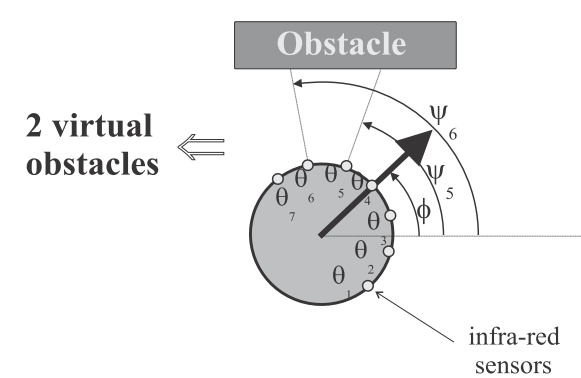
\includegraphics[width=0.55\textwidth]{./img/fig2-obstacles.png}
  \caption{Obstacle avoidance behavior: sensor placement}%
\label{fig:fig2-obs}
\end{figure}

The strategy adopted consists in assuming that each sensor $i$ specifies a
virtual obstacle in the direction $\psi_{obs,i}$ if an obstruction is detected
in that direction. Each virtual obstacle is modelled by a repulsive force
centered in the direction the respective sensor points out:
\begin{equation}
  \label{eq:24}
  f_{obs,i}(\phi) = \lambda_{obs,i} (\phi -\psi_{obs,i}) \exp \Big(-\frac{(\phi - \psi_{obs,i})^2}{2 \sigma_i ^2} \Big)
  = \lambda_{obs,i} (- \theta_i) \exp \Big(-\frac{(- \theta_i)^2}{2 \sigma_i ^2} \Big)
\end{equation}
It must be pointed out that the only diference $\phi - \psi_{obs,i} = - \theta_i$,
which is fixed and known, goes into the heading direction dynamics, thus
yielding the calibration of the system in respect to the external reference axis
irrelevant.

The strength of the repulsion, $\gls{lambda-obs-i}$, from the virtual obstacle at
direction $\gls{psi-obs-i}$, is a decreasing function of the sensed distance, $\gls{d-i}$ ---
high for small distances and low for high distances and null for $d_i \ge
d_{max}$ (sensor range maximum) --- which can be exponential:
\begin{equation}
  \label{eq:25}
  \lambda_{obs,i} = \beta_1 \exp \Big( -\frac{d_i}{\beta_2} \Big)
\end{equation}
where $\gls{beta1}$ determines the maximum strenght of repulsion and $\gls{beta2}$ is
the decay rate of the repulsion force with the distance increase.

The angular range over which the force-let exerts its repulsive effect, 
$\gls{sigma-i}$ is given by:
\begin{equation}
  \label{eq:26}
  \sigma_{i} = \arctan \Bigg( \tan \Big(\frac{\Delta \theta}{2} \Big ) + 
  \frac{R_{robot}}{R_{robot} + d_i}\Bigg)
\end{equation}
where $\gls{delta-theta}$ is the angular distance between adjacent sensors (sensor
sector), $R_{robot}$ is the radius of the robot, and $d_i$ is the distance
estimated by the sensor $i$.

The contributions from all the sensors are summed, thus, yielding the overall
obstacle avoidance dynamics as follows:
\begin{equation}
  \label{eq:27}
 \frac{d \phi}{dt} = \gls{F-obs}(\phi) = f_{obs}(\phi) + f_{stoch}
%\quad N = nr of sensors
\end{equation}
where $N$ is the number of sensors, in this case, $\gls{N} = 11$, $\gls{f-obs}$ is the
total repulsion force due to all obstacles contributions (Eq.~(\ref{eq:35})),
and $f_{stoch}$ is
the stochastic force given by Eq.~(\ref{eq:6}).
\begin{equation}
  \label{eq:35}
  f_{obs} (\phi) = \sum_{i = 1}^N \gls{f-obs-i}(\phi) 
\end{equation}

\section{Analytical study}%
\label{sec:analytical-study-obs}
In this section the analytical study of the overall obstacle avoidance dynamics
(Eq.~(\ref{eq:27})) is performed. The fixed points are determined and its
stability assessed. The phase portraits and bifurcation diagram are
plotted. Lastly, the range of admissible values for the parameter $\beta_1$ and
the repulsion time constant are computed.

\subsection{Fixed points}%
\label{sec:fixed-points-obs}
The fixed points for the dynamic system given by Eq.~(\ref{eq:27}) are computed,
considering that only one obstruction is detected, i.e.:
\begin{equation}
  \label{eq:28}
 \frac{d \phi}{dt} = F_{obs}(\phi) = f_{obs,1}(\phi)
\end{equation}
%
The fixed points are the constant solutions of the dynamic system, i.e.:
\begin{equation}
  \label{eq:29}
\begin{array}{ll}
  \left. \frac{d \phi}{dt}\right|_{\phi = \phi^*} = f_{obs, 1}(\phi^*) = 0 
\quad \leftrightarrow \quad 
  \lambda_{obs,1} (\phi^* -\psi_{obs,1}) \exp \Big(-\frac{(\phi^* - \psi_{obs,1})^2}{2 \sigma_i ^2} \Big) = 0 
\quad \leftrightarrow \quad 
\\ 
\quad \leftrightarrow \quad (\lambda_{obs,1} = 0 \vee \phi^* - \psi_{obs,1} = 0 \vee  \exp \Big(-\frac{(\phi^* - \psi_{obs,1})^2}{2 \sigma_i ^2} \Big) = 0) \wedge \lambda_{obs,i} \ne 0
\\ 
\quad \leftrightarrow \quad 
\boxed{\phi^* = \psi_{obs,1}}
\end{array}
\end{equation}
There is one fixed point at $\phi^* = \psi_{obs,1}$.

\subsection{Stability}%
\label{sec:stability-obs}
The determination of the stability of fixed points is useful to understand its
qualitative behavior. It can be determined analytically evaluating the slope in
the vicinity of the fixed point. First, let one compute the derivative:
\begin{equation}
  \label{eq:30}
\begin{array}{ll}
  f'_{obs, 1}(\phi) = \frac{d f_{obs,1}(\phi)}{d \phi} = 
\frac{d}{d \phi} \Bigg( \lambda_{obs,1} (\phi -\psi_{obs,1}) \exp \Big(-\frac{(\phi - \psi_{obs,1})^2}{2 \sigma_i ^2} \Big) \Bigg)
\quad = \quad 
\\ 
= 
\frac{d}{d \phi} \Big(\phi -\psi_{obs,1}\Big) \lambda_{obs,1} \exp \Big(-\frac{(\phi - \psi_{obs,1})^2}{2 \sigma_i ^2} \Big) +
\frac{d}{d \phi} \Bigg( \exp \Big(-\frac{(\phi - \psi_{obs,1})^2}{2 \sigma_i ^2} \Big) \Bigg) \lambda_{obs,1} (\phi^* -\psi_{obs,1}) 
\leftrightarrow
\\ 
\quad \leftrightarrow \quad 
  f'_{obs, 1} (\phi) = \lambda_{obs,1} \exp \Big(-\frac{(\phi - \psi_{obs,1})^2} {2 \sigma_i ^2} \Big) \Big(1 - \frac{(\phi -\psi_{obs,1})^2}{\sigma_1 ^2} \Big) 
\end{array}
\end{equation}
Then, computing the derivative at the fixed point yields:
\begin{equation}
  \label{eq:31}
  \begin{array}{ll}
  f'_{obs, 1} (\phi^*) = f'_{obs, 1} (\psi_{obs,1}) =
  \lambda_{obs,1} \exp \Big(-\frac{(\psi_{obs,1} - \psi_{obs,1})^2} {2 \sigma_i ^2} \Big) \Big(1 - \frac{(\psi_{obs,1} -\psi_{obs,1})^2}{\sigma_1 ^2} \Big) 
\\
\quad \leftrightarrow \quad 
    \boxed{ f'_{obs, 1} (\phi^*) = \lambda_{obs,1}}
  \end{array}
\end{equation}

Analyzing the possible cases for the slope at the fixed point, it can be
observed that:
\begin{equation}
  \label{eq:22}
  m = \left\{
\begin{array}{ll}
      < 0 , & \lambda_{obs} < 0 \quad \rightarrow \quad \mathrm{attractor} \\
      > 0 , & \lambda_{obs} > 0 \quad \rightarrow \quad \mathrm{repeller} \\
      = 0 , & \lambda_{obs} = 0 \quad \rightarrow \quad \mathrm{inconclusive} \\
\end{array} 
\right. 
\end{equation}
The desired heading direction dynamics requires that a repeller is placed in
the obstacle direction, i.e. $\phi^* = \psi_{obs,1}$ is an repeller, thus
$\lambda_{obs} > 0$. The repulsion time for the repeller is given by:
\begin{equation}
  \label{eq:23}
 \tau_{obs,1} = \frac{1}{| f'_{obs,1}(\phi^*) |} \quad \leftrightarrow \quad \boxed{\tau_{obs,1} = \frac{1}{\lambda_{obs,1}}}
\end{equation}

\subsection{Phase portraits}%
\label{sec:phase-portraits-obs}
Fig.~\ref{fig:obs-phase-portraits} illustrates the phase portraits for the
dynamic system responsible for the obstacle avoidance behavior. It can be
observed that for $\lambda_{obs} < 0$, $\phi^* = \psi_{obs}$ is an attractor and
conversely if $\lambda_{obs} < 0$, $\phi^* = \psi_{obs}$ is an repeller. As
previously mentioned the latter represents the desired behavior.
%
\begin{figure}[!hbt]
\centering
\begin{subfigure}{.5\textwidth}
  \centering
  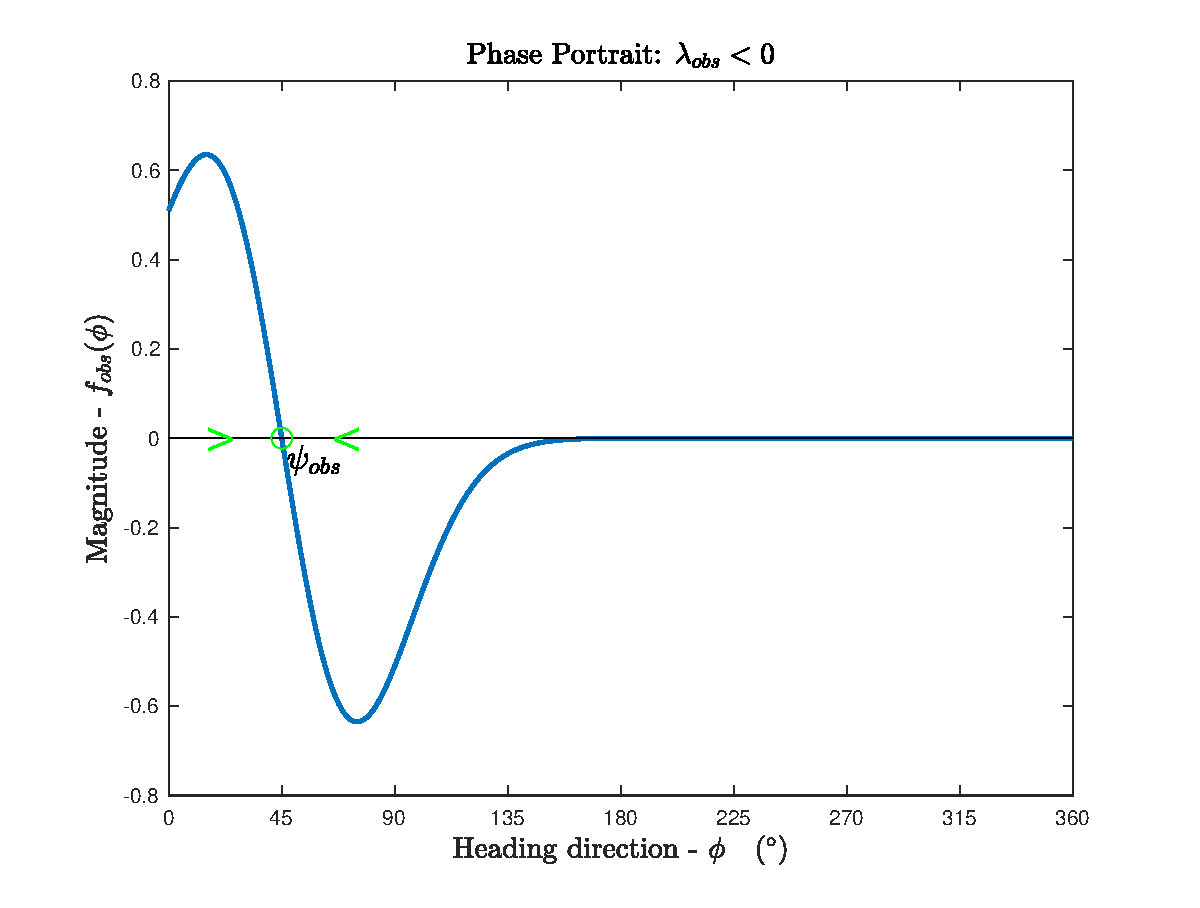
\includegraphics[width=1.0\textwidth]{./img/obs-phase-portrait-1.eps}
  \caption{$\lambda_{obs} < 0$: attractor}%
  \label{fig:obs-phase-port-1}
\end{subfigure}%
\begin{subfigure}{.5\textwidth}
  \centering
  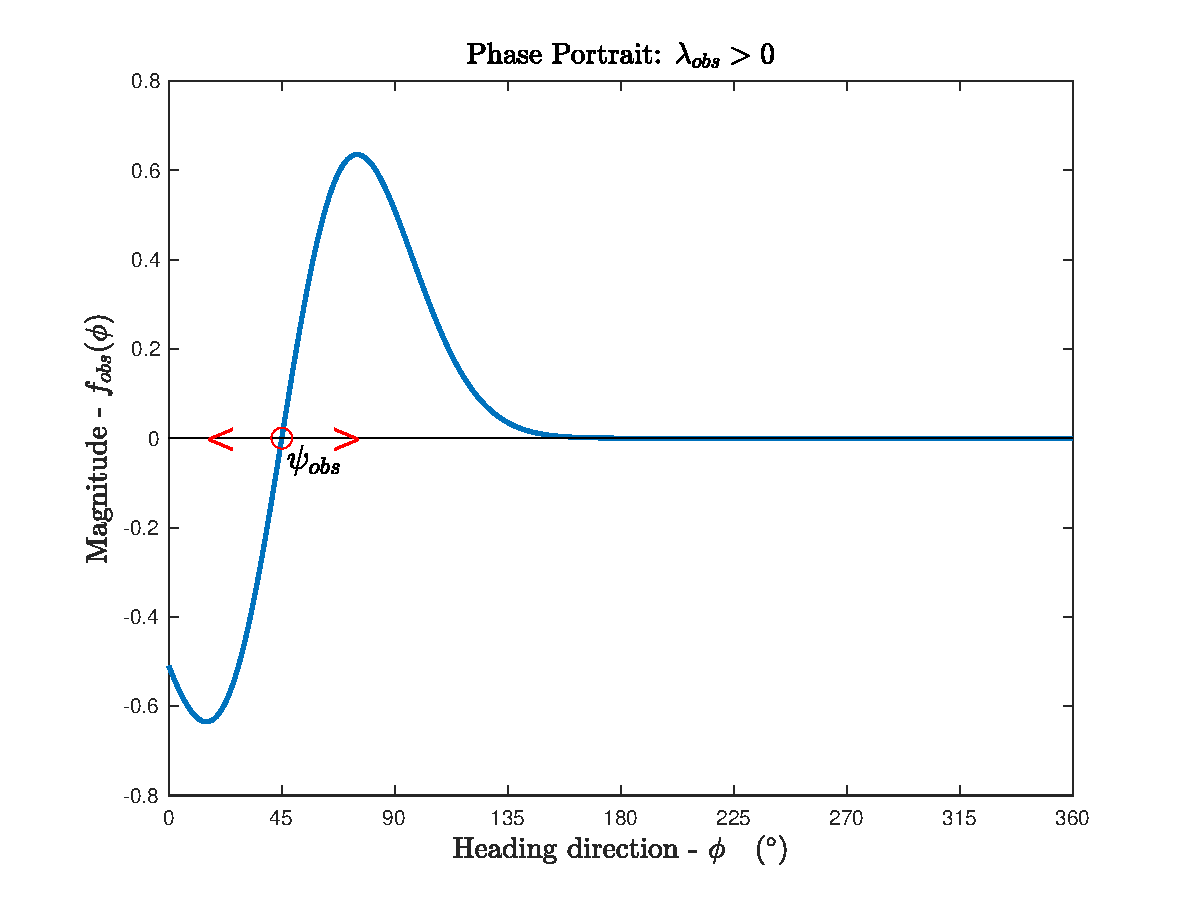
\includegraphics[width=1.0\textwidth]{./img/obs-phase-portrait-2.eps}
  \caption{$\lambda_{obs} > 0$: repeller}%
  \label{fig:obs-phase-port-2}
\end{subfigure}
\caption{Obstacle avoidance behavior: Phase portraits}%
\label{fig:obs-phase-portraits}
\end{figure}
%
\subsection{Bifurcation diagram}%
\label{sec:bifurcation-diagram-obs}
Fig.~\ref{fig:1-4-obs-bifurcation-diag} depicts the bifurcation diagram for the
target acquisition dynamic system, as a function of the parameter
$\lambda_{obs}$ $( \psi_{tar} \in [0, 2 \pi[ )$:
\begin{itemize}
\item $\lambda_{obs} < 0$: the fixed point $\phi^*$ is asymptotically stable.
\item $\lambda_{obs} > 0$: the fixed point $\phi^*$ is unstable.
\end{itemize}
%
$\lambda_{obs} = 0$ is a bifurcation point. This represents a transcritical bifurcation as there is an exchange in the
stability in the fixed point.
%
% Bifurcation diagram
\begin{figure}[!hbt]
\centering
    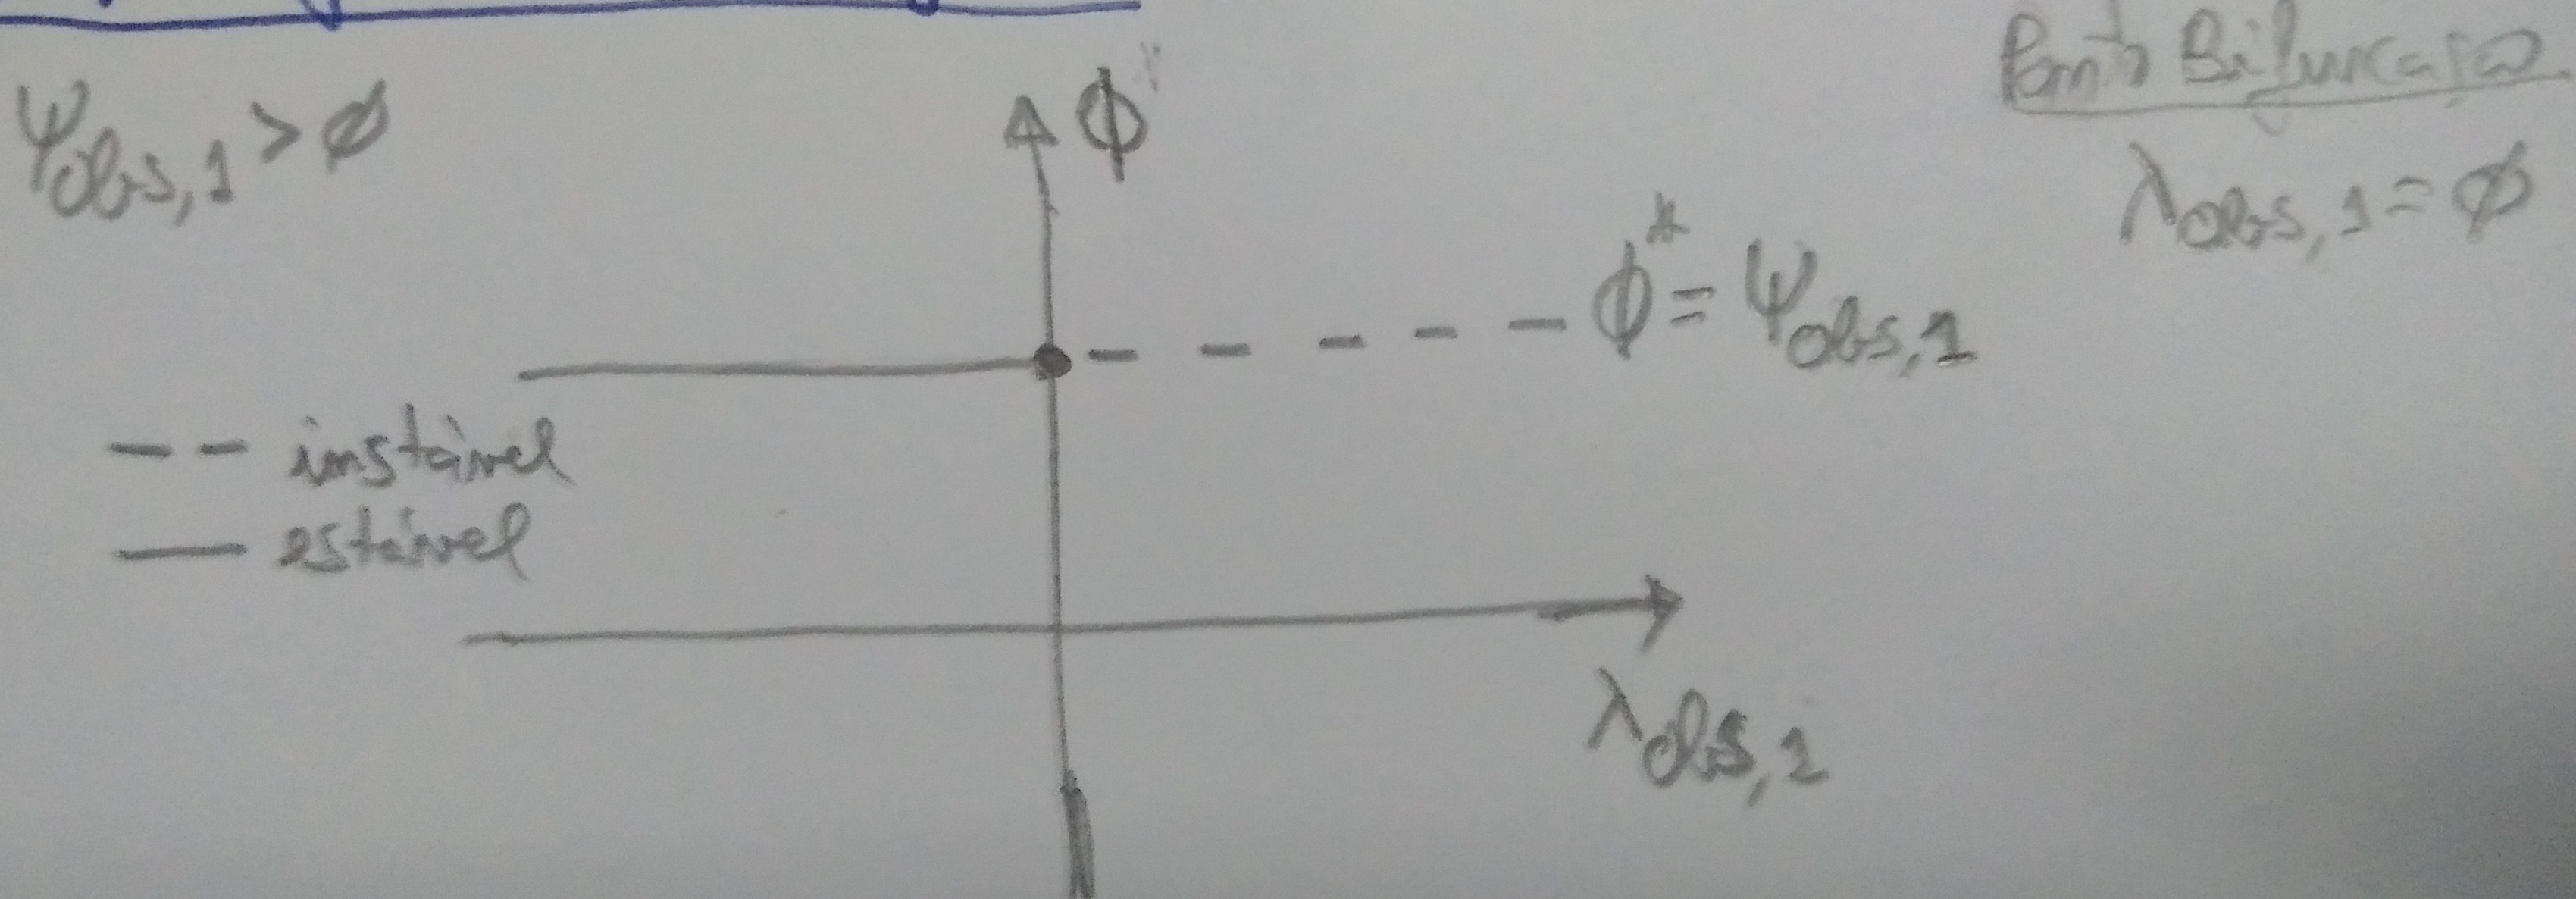
\includegraphics[width=0.6\textwidth]{./img/obs-bifurcation-diag.jpg}
  \caption{Obstacle behavior: Bifurcation diagram}%
\label{fig:1-4-obs-bifurcation-diag}
\end{figure}
%
%
\subsection{Range of values for $\beta_1$}%
\label{sec:range-values-beta1}
The parameter $\beta_1$ represents the maximum strength of the repulsive
forcelet, given by:
\begin{equation}
  \label{eq:32}
  \beta_1 = \max( \lambda_{obs,i} ) = \frac{1}{\min( \tau_{obs,i} )}
\end{equation}
i.e., is the inverse of the minimum time constant, $\gls{tau-obs-i}$, between all sensors.
The minimum time constant must be much greater than the Euler's step, $\Delta
t$, and considering reasonable boundaries, one has: 
\begin{equation}
  \label{eq:33}
 5 \Delta t < min(\tau_{obs}) <  10 \Delta t 
\quad \leftrightarrow \quad  
 \frac{1}{10  \Delta t} < \beta_1 <  \frac{1}{5 \Delta t}
\end{equation}
%
\subsection{Repulsion time constant}%
\label{sec:repuls-time-const}
This was previously calculated (see Section~\ref{sec:stability-obs}). 
%It should be noted, however, that for the overall obstacle avoidance dynamics,
%the repulsion time constant is calculated as the sumation of all time constants:
%\begin{equation}
%  \label{eq:33}
% m = \sum_{i = 1}^N {f'_{obs, i} (\phi_i^*)} = \sum_{i = 1}^N {\lambda_{obs, i}}= \lambda_{tot}
%\quad \leftrightarrow \quad
%\tau_{obs} = \frac{1}{\lambda_{tot}} = \frac{1}{\sum_{i=1}^N{\tau_{obs,i}}}
%\end{equation}
%
%
\section{Implementation}%
\label{sec:implementation-obs}
In this section, the implementation of the nonlinear dynamic system for obstacle
avoidance and simulation in CoppeliaSim using scenario
\texttt{MobileRobotDyn\_Tar\_Obs.ttt} is described for several different environment
scenarios. This aided the comprehension of the influence of several parameters
and enabled its successfull tuning, yielding the desired obstacle avoidance
behavior for the robot.

The first step of the implementation is to convert the first order differential
equation into an algebraic recursive equation by applying the forward Euler's
method in a discrete form:
\begin{equation}
  \label{eq:34}
  \phi(t + \Delta t) = \phi(t) + \Delta t F_{obs}(\phi), \qquad \phi(t_0) = \phi_0
\end{equation}
where $\Delta t$ is the Euler's step --- the incremental timestep applied to
the recursive equation and $F_{obs}(\phi)$ is given by Eq.~(\ref{eq:27}).
Simplying, both components of the dynamic system, $f_{obs}$ and $f_{stoch}$ can be
computed separately using Eqs.~(\ref{eq:35}) and~(\ref{eq:6}) and added,
yielding the complete dynamic system as given by Eq.~(\ref{eq:27}). Next, the
angular velocity of the vehicle can be determined, noting that $\omega _{robot}
= d \phi /dt$, i.e., equal to the complete vector field.

For smooth variation of the heading direction the
Euler's step must be significantly smaller than the minimum time constant (in
this case, the repulsion time), i.e., $\Delta t \ll \min(\tau _{obs})$, as
previously determined.

Next, for each sensor are computed the contribution to the repulsive force-let,
namely the direction the obstacle is seen, $\psi_{obs,i}$, magnitude of repulsion,
$\lambda_{obs,i}$, the range of repulsion, $\sigma_i$, and the effective
contribution to the repulsive forcelet, $f_{obs,i}$. The latter is accumulated,
yielding $f_{obs}$.

Finally, linear velocity is defined, and, if desired a stop criterion for the
distance to target. Then, the values of the angular and linear velocities of the
robot can be passed as setpoints to the low-level code responsible for
controlling these control variables.

Summarizing, the pseudocode for the obstacle avoidance behavior is as follows:
\begin{enumerate}
\item Initialize robot: retrieve simulation timestep and robot characteristics
\item Set initial values (linear and angular velocities) and set robot's initial
  pose ($x_{robot}, y_{robot}, \phi_{robot}$)
\item Define global parameter values: $N$, $\beta_2$, $Q$
\item Compute angular sector: $\Delta \theta = \theta_{obs,2} - \theta_{obs,1}$
\item Initialize target
\item While target <= targetNr
  \begin{enumerate}
  \item Exchange information with the simulator
  \item Get vehicle's pose, target position and simulation timestep
  \item Trigger a simulation step
  \item Processing step
    \begin{enumerate}
    \item Set parameters values: $\tau_{tar}, \lambda_{tar}, Q$
    \item For each sensor, compute the contribution of the repulsive forcelet
      \begin{enumerate}
      \item Compute $\psi_{obs,i}$, $\lambda_{obs,i}$, $\sigma_i$
      \item Compute $f_{obs,i}$
      \item Compute $f_{obs} = f_{obs} + f_{obs,i}$
      \end{enumerate}
    \item Compute $f_{obs}$ and $f_{stoch}$
    \item Compute resultant vector field $f_{total}$ and assign it to angular
      velocity
    \item Set linear velocity
    \item Define stop criterion for target distance (if desired)
    \end{enumerate}
  \item View dynamics: plot the obstacle avoidance dynamics
  \item Set robot's angular and linear velocities
  \end{enumerate}
\item Terminate simulation and cleanup
\end{enumerate}

As a result, the following generic Matlab code was implemented (Listing~\ref{lst:program-dyn-obs}):
% program_dyn_tar.m (generic)
\lstinputlisting[language=matlab, caption={Generic implementation of obstacle
  avoidance behavior (not tuned)},label=lst:program-dyn-obs,
style=custom-matlab]{./listing/program_dyn_obs.m}%

\subsection{Scenario 1}%
\label{sec:scenario-1-obs}
The obstacles were placed at a distance of 0 cm between each other to form a
wall (no gap). The robot was
placed in the middle of the arena and facing the wall at a distance of 100 cm. The stochastic force was
reset (null variance --- $Q = 0$). The robot moves at a constant linear velocity
of 20 cm/s, which is a reasoable value. The  parameter $\beta_2 = 20$ was fixed
and $\beta_1$ was increased until the robot avoids collision with the wall.
Then, for each value of $\beta_1$, the contribution of each sensor and the
resultant obstacle avoidance dynamics were observed.

$\beta_1$ is related to $\min(\tau_{obs,i})$ (Eq.~(\ref{eq:32})), thus,
\texttt{tau\_obs\_min} was set, starting from $10 \Delta t$ and
decremented at unit steps. Fig.~\ref{fig:obs-2-1-arena-fail} illustrates the
simulation for \texttt{tau\_obs\_min} = $5 \Delta t$, where a collision occurs
with a wall (robot becomes red). 
%
\begin{figure}[!hbt]
\centering
    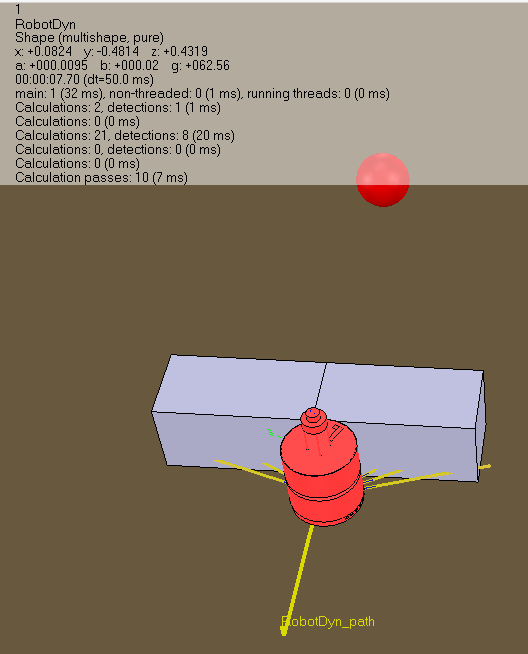
\includegraphics[width=0.55\textwidth]{./img/obs-2-1-arena-fail.png}
  \caption{Obstacle avoidance behavior: \texttt{tau\_obs\_min} = $5 \Delta t$}%
\label{fig:obs-2-1-arena-fail}
\end{figure}

Conversely, in
Fig.~\ref{fig:obs-2-1-arena-success} is illustrated the final state of the first
compliable value of $beta_1$ for collision-free path (\texttt{tau\_obs\_min} =
$4 \Delta t$), as indicated by the auxiliary text 
(see also Video \href{run:./videos/obs-2-1.mp4}{./videos/obs-2-1.mp4}). 
In the obstacle avoidance
dynamics plot it can be observed that, in the final state depicted, the heading
direction is very far appart from the repeller, as expected. 
%
\begin{figure}[!hbt]
\centering
    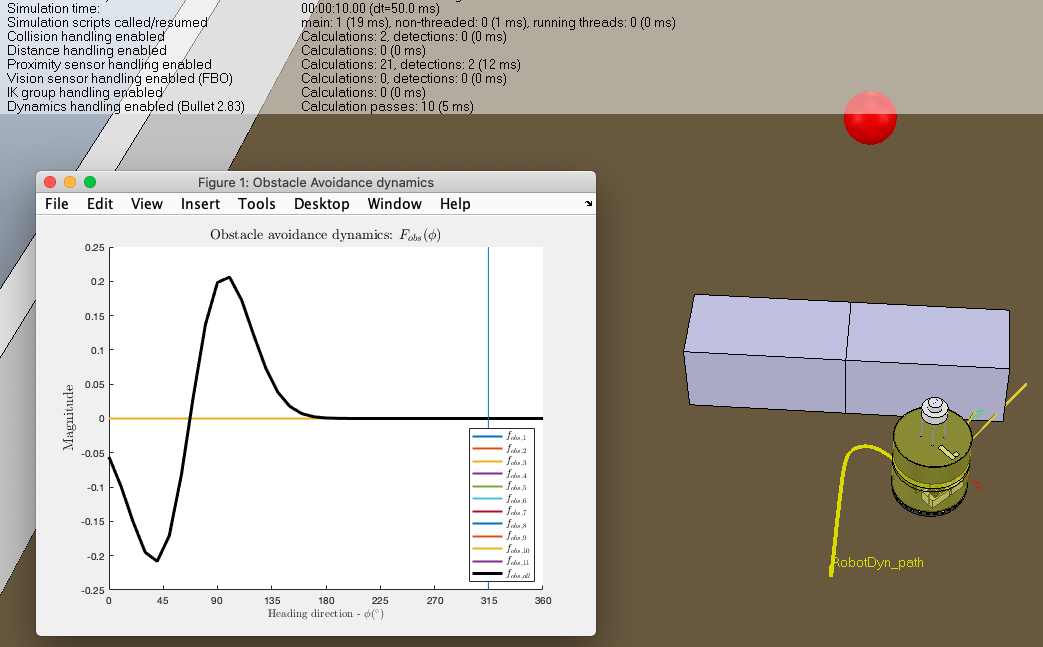
\includegraphics[width=0.9\textwidth]{./img/obs-2-1-arena-success.png}
  \caption{Obstacle avoidance behavior: \texttt{tau\_obs\_min} = $4 \Delta t$ (final state)}%
\label{fig:obs-2-1-arena-success}
\end{figure}

The deviation from
the obstacles only happened when the strenght of the repeller was
sufficiently high to induce significant angular velocities, which for this case,
started at $\omega = d\phi/dt = -0.5$ rad/s and hit its maximum at approximately
$\omega = -3$ rad/s, representing an counterclockwise turn. It is important to note, however, that this calibration for
collision-free path of the parameter $\beta_1$ is dependent on the value of the
linear velocity, as the system may not have time to react to it --- the higher
the value of the linear velocity (constant), the lower the value of
\texttt{tau\_obs\_min} needs to be. On the other hand, the linear velocity
should decrease with the distance to the obstacles, which could be modelled as a
dynamic system, e.g., the one in Eq.~(\ref{eq:12}).

Fig.~\ref{fig:obs-scenario1-facing-front} shows in more detail the obstacle
avoidance dynamics plot, used as an aiding tool, with the robot direction
direction still facing the wall, i.e., $\phi = \psi_{obs}$. It can be seen that
5 sensors are detecting the obstacles, yielding a stronger reppeller in that
direction, but still insufficient for significant direction change.
%
\begin{figure}[!hbt]
\centering
    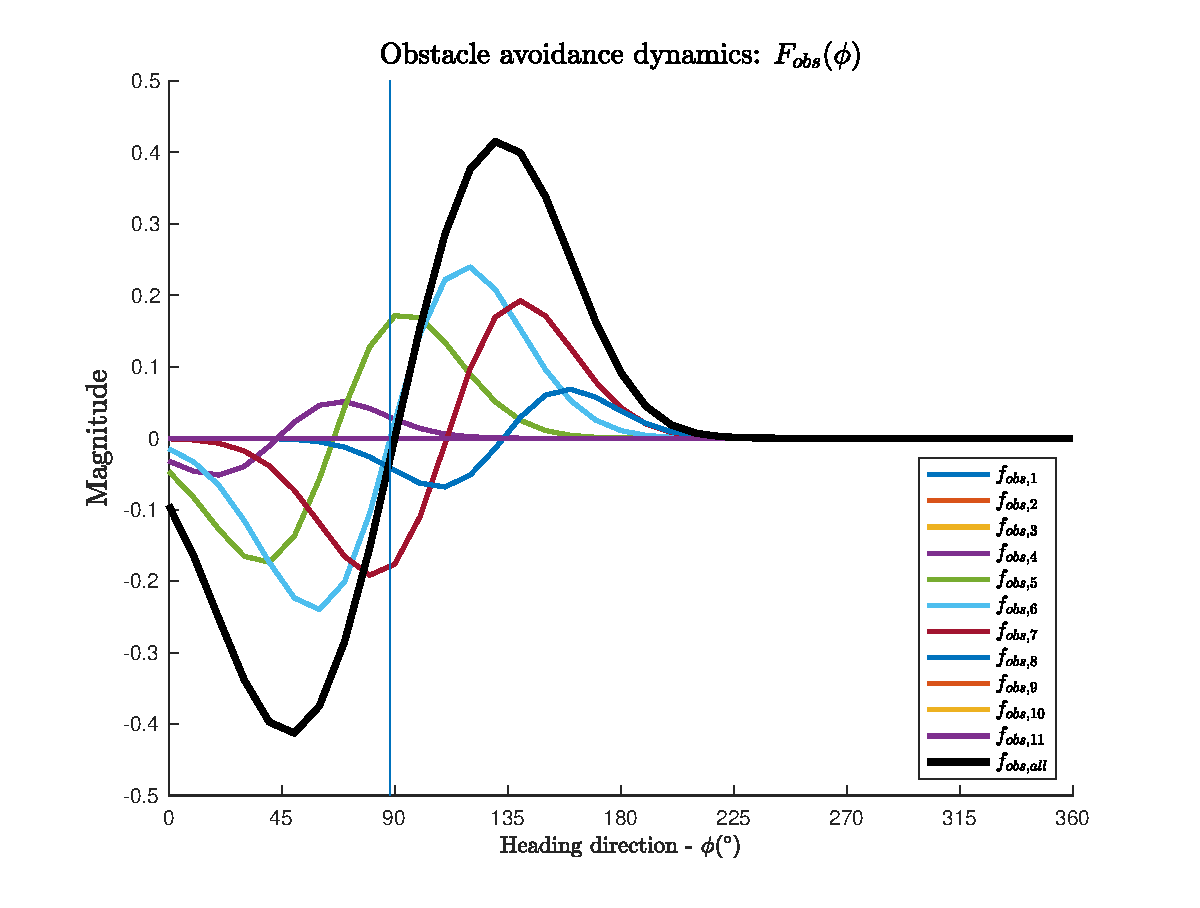
\includegraphics[width=0.7\textwidth]{./img/obs-scenario1-facing-front.eps}
  \caption{Obstacle avoidance behavior: dynamics --- \texttt{tau\_obs\_min} = $4 \Delta t$}%
\label{fig:obs-scenario1-facing-front}
\end{figure}

The addition of noise to the dynamic system was unnecessary, as there is a
slight bias from sensors readings, due to uneven obstacle detection by all
sensors --- the leftmost sensors did not detect the obstacles initially, whereas
the rightmost did. This slight bias for obstacles detection is responsible for
the counterclockwise turn, rendering it unnecessary to incorporate noise for the
robot to deviate from the obstacles, albeit the heading direction initially sits in a repeller.
%
%
\subsection{Scenario 2}%
\label{sec:scenario-2-obs}
The obstacles were now placed at a 10 cm gap between each other, 
and the robot was
placed in the middle of the arena facing the gap at a distance of 100 cm. 
The remaining conditions from scenario 1 remained unchanged.

First, the system was simulated with the previous value of $\beta_1$ to assess
the system's behavior (Fig.~\ref{fig:obs-2-2-1}). It can be seen that the robot
collides with an obstacle in the attempt to deviate from it, as the heading
direction still remains inside the influence of repellers. 
%
\begin{figure}[!hbt]
\centering
    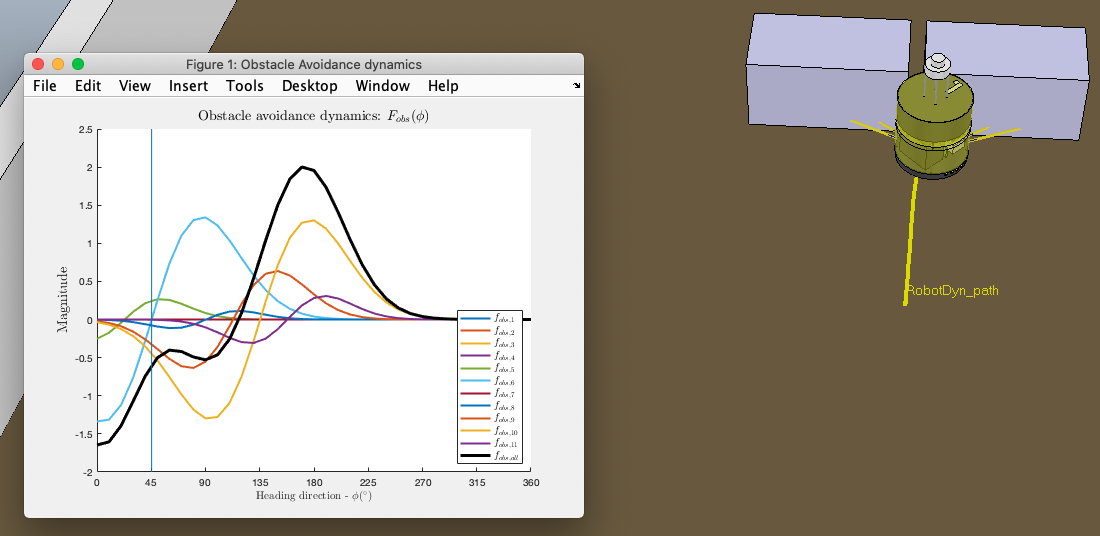
\includegraphics[width=0.7\textwidth]{./img/obs-2-2-1.png}
  \caption{Obstacle avoidance behavior: dynamics --- \texttt{tau\_obs\_min} = $4
    \Delta t$, gap = 10 cm}%
\label{fig:obs-2-2-1}
\end{figure}

It does not detect obstacles in most of the path in the most central sensor, as it moves forward, due to the gap, which was
the most strong contribution. When the contributions of the other sensors are
high enough to trigger robot's rotation, the robot starts to rotate
(counterclockwise, in this case), but the dynamics is not fast or strong enough
to avoid the obstacle.

The value of parameter $\beta_1$ was then retuned to avoid collisions with the
obstacles, following the same procedure, i.e., decrementing
\texttt{tau\_obs\_min}. Fig.~\ref{fig:obs-2-2-2} illustrates the first
collision-free path of the robot with the new environment conditions, occurring
at \texttt{tau\_obs\_min} = $3.5 \Delta t$ (see also Video
\href{run:./videos/obs-2-2.mp4}{./videos/obs-2-2.mp4}).
%
\begin{figure}[!hbt]
\centering
    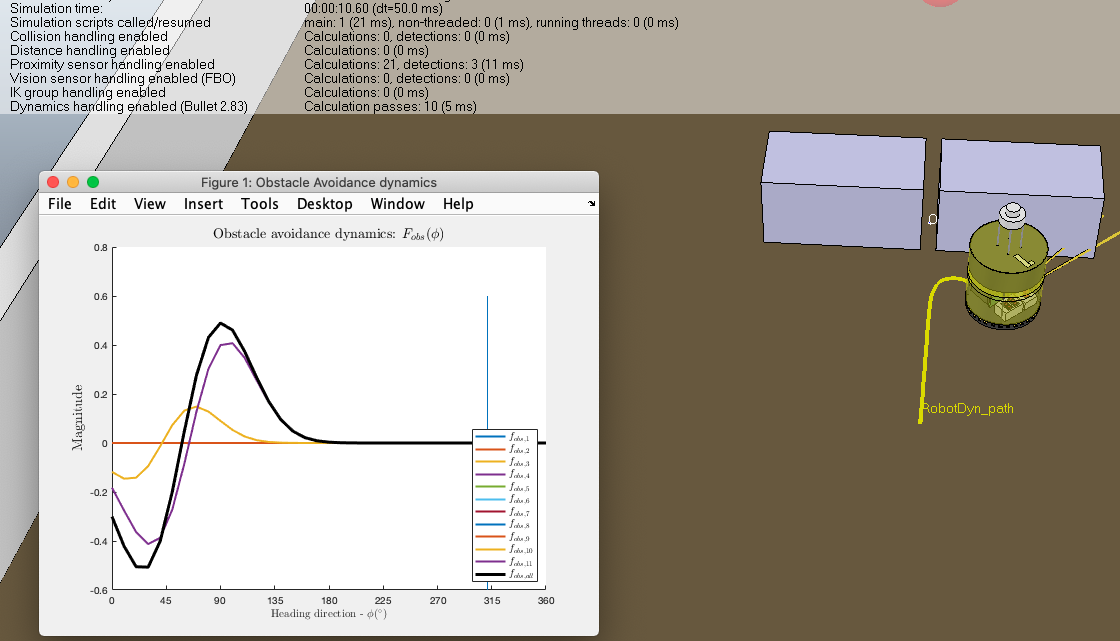
\includegraphics[width=0.7\textwidth]{./img/obs-2-2-2.png}
  \caption{Obstacle avoidance behavior: dynamics --- \texttt{tau\_obs\_min} =
    $3.5 \Delta t$, gap = 10 cm}%
\label{fig:obs-2-2-2}
\end{figure}
%
\subsection{Scenario 3}%
\label{sec:scenario-3-obs}
In this scenario several simulations are performed for different gaps between
obstacles, namely 20--80 cm, with a 10 cm span. Fig.~\ref{fig:obs-2-3-50cm}
illustrates the first case where the robot can move between the obstacles, which
occurs for a distance gap of 50 cm between them.
(see also Video
\href{run:./videos/obs-2-3-50cm.mp4}{./videos/obs-2-3-50cm.mp4}). Fig.~\ref{fig:obs-2-3-50cm-2}
shows that for a 50 cm gap, in the situation depicted in Fig.~\ref{fig:obs-2-3-50cm-1}, the heading direction has an attractor, instead of a
repeller (0--40 cm), and two repellers at approximately 60$^{\circ}$ and 120$^{\circ}$.
%
\begin{figure}[!hbt]
\centering
\begin{subfigure}{.5\textwidth}
  \centering
  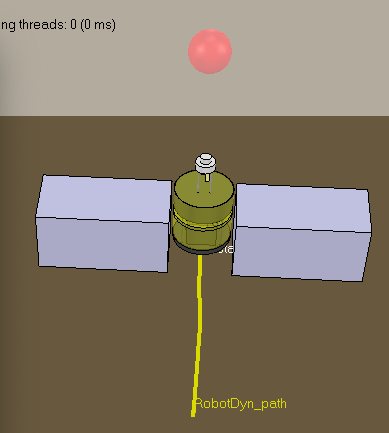
\includegraphics[width=0.7\textwidth]{./img/obs-2-3-50cm-1.png}%
  \caption{Simulation}%
\label{fig:obs-2-3-50cm-1}
\end{subfigure}%
\begin{subfigure}{.5\textwidth}
  \centering
  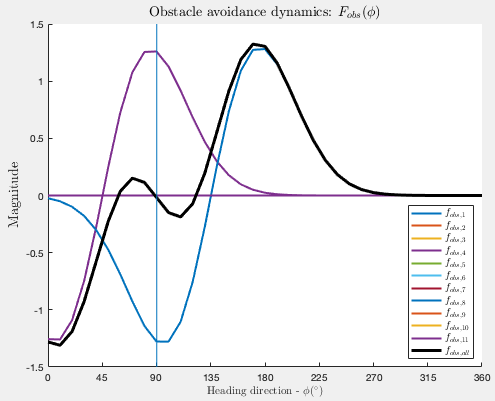
\includegraphics[width=1.0\textwidth]{./img/obs-2-3-50cm-2.png}%
  \caption{Dynamics}%
\label{fig:obs-2-3-50cm-2}
\end{subfigure}
  \caption{Obstacle avoidance behavior: dynamics --- \texttt{tau\_obs\_min} =
    $3.5 \Delta t$, gap = 50 cm}%
\label{fig:obs-2-3-50cm}
\end{figure}
%
\subsection{Bifurcation analysis}%
\label{sec:bifurcation-analysis-obs}
As indicated in Section~\ref{sec:scenario-3-obs}, the heading direction dynamics
exhibits different qualitative behavior --- the stability of the fixed
points varies --- starting from gap = 50 cm. This corresponds to a bifurcation
point, representing the distance below which the robot
(with diameter 45 cm) cannot pass between the two obstacles. For gap < 50 cm, the planning dynamics has an reppeller
at the heading direction $\phi = \pi/2$, and for gap > 50 this reppeller becomes
asymptotically stable (i.e., an attractor).

\subsection{Influence of parameter $\beta_2$}%
\label{sec:infl-param-beta2}
The parameter $\beta_2$ is the decay rate of the repulsion force with the
distance increase. Thus, to test this, $\beta_2$ was varied and simulated in the
conditions of scenario 1, and the resulting repulsion magnitude
$\lambda_{obs,i}$ computed (see Fig.~\ref{fig:obs-2-5}). 
%
\begin{figure}[!hbt]
\centering
\begin{subfigure}{.5\textwidth}
  \centering
  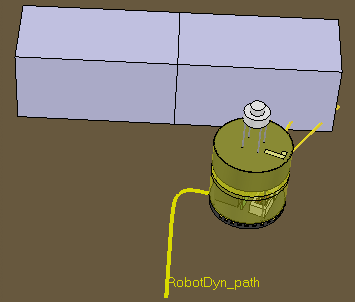
\includegraphics[width=0.7\textwidth]{./img/obs-2-5-beta2-50.png}%
  \caption{$\beta_2 = 50$}%
\label{fig:obs-2-5-beta-2-50}
\end{subfigure}%
\begin{subfigure}{.5\textwidth}
  \centering
  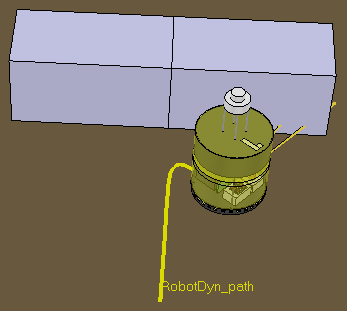
\includegraphics[width=0.7\textwidth]{./img/obs-2-5-beta2-15.png}%
  \caption{$\beta_2 = 15$}%
\label{fig:obs-2-5-beta2-15}
\end{subfigure}
  \caption{Obstacle avoidance behavior: influence of parameter $\beta_2$}%
\label{fig:obs-2-5}
\end{figure}

For increasing values of $\beta_2$ (Fig.~\ref{fig:obs-2-5-beta-2-50}), the decay rate
diminishes, maintaining the repulsive effect significantly for
a wider distance range --- the robot starts to rotate farther away from the obstacles.
Conversely, for decreasing values of $\beta_2$ (Fig.~\ref{fig:obs-2-5-beta2-15}), the decay rate
increases, maintaining the repulsive effect significantly for
a narrow distance range --- the robot starts to rotate closer to the obstacles.

\subsection{Influence of noise}%
\label{sec:influence-noise-obs}
The influence of noise was tested, varying the value of the magnitude of
gaussian white noise, $Q$ (see Fig.~\ref{fig:obs-2-6}).
%
\begin{figure}[!hbt]
\centering
\begin{subfigure}{.5\textwidth}
  \centering
  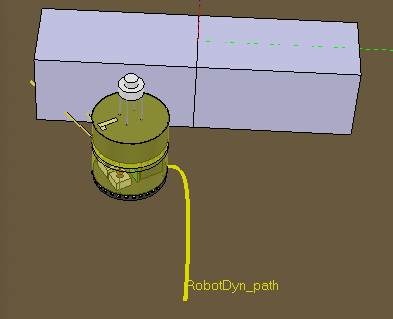
\includegraphics[width=0.76\textwidth]{./img/obs-2-6-Q-005.png}%
  \caption{$\beta_2 = 15, Q = 0.05$}%
\label{fig:obs-2-6-Q-005}
\end{subfigure}%
\begin{subfigure}{.5\textwidth}
  \centering
  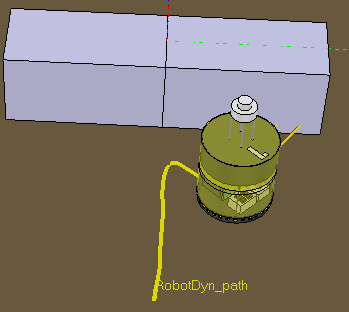
\includegraphics[width=0.7\textwidth]{./img/obs-2-6-Q-05.png}%
  \caption{$\beta_2 = 15, Q = 0.5$}%
\label{fig:obs-2-6-Q-05}
\end{subfigure}
  \caption{Obstacle avoidance behavior: influence of noise}%
\label{fig:obs-2-6}
\end{figure}

Comparing Fig.~\ref{fig:obs-2-6-Q-005} with Fig.~\ref{fig:obs-2-5-beta2-15}, it
can be seen that the mere introduction of noise induced a different qualitative
behavior with the decision of turning left instead of right,
respectively. Additionally, in Fig.~\ref{fig:obs-2-6-Q-05}, it can be seen the
magnitude of noise should be maintained fairly low, as it may introduce jitter
into the system, depicted by the less `clean' path. Thus, the noise should be
sufficient to enough to guarantee the escape from the repellers within a time
limit, in case the system is initially placed there.

\subsection{Scenario 4}%
\label{sec:scenario-4-obs}
Fig.~\ref{fig:obs-2-7} illustrates scenario 4, composed of several obstacles
that the robot must avoid. It can be observed that the robot is able to avoid
all obstacles, as expected.

\begin{figure}[!hbt]
\centering
    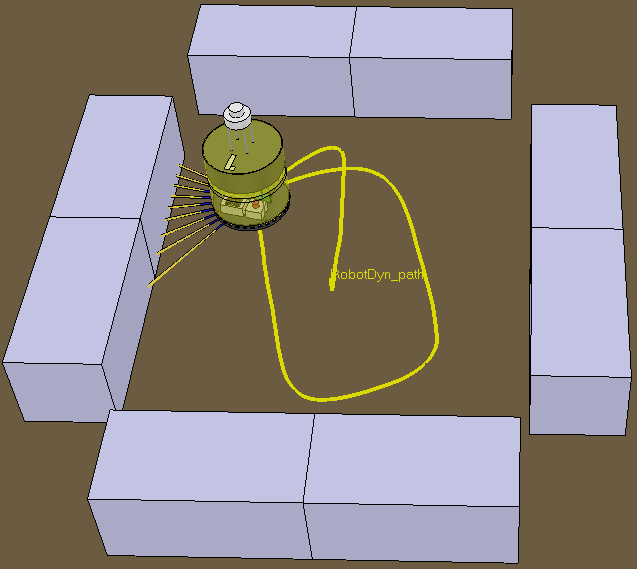
\includegraphics[width=0.6\textwidth]{./img/obs-2-7.png}
  \caption[Obstacle avoidance behavior: Simulation with several obstacles]{Obstacle avoidance behavior: Simulation with several obstacles --- \texttt{tau\_obs\_min} =
    $3.5 \Delta t$, Q = 0.05, $\beta_2 = 20$}%
\label{fig:obs-2-7}
\end{figure}
%%% Local Variables:
%%% mode: latex
%%% TeX-master: "../../dissertation"
%%% End:
